\frame
{
\frametitle{Sintonización Manual}
\framesubtitle{Configuración Inicial}
\begin{itemize}
    \item \texttt{POP = 20}
    \item \texttt{GENS = 200}
    \item \texttt{clonationFactor = 0.4}
    \item \texttt{clonationRate = 0.5}
    \item \texttt{replaceRate = 0.6}
\end{itemize}

}

\frame
{
\frametitle{Sintonización Manual}
\framesubtitle{Instancias escogidas}
\begin{center}
    \begin{tabular}{|l|c|}
    \hline
    \textbf{Instancia} & \textbf{Mejor Fitness conocido} \\\hline
    \texttt{pb\_200\_01.txt} & 0 \\\hline
    \texttt{pb\_200\_09.txt} & 10 \\\hline
    \texttt{pb\_200\_10.txt} & 19 \\\hline
    \end{tabular}
\end{center}
}

\frame
{
\frametitle{Sintonización Manual}
\framesubtitle{Prueba 1}
\vspace{1cm}
\begin{center}
    Tamaño de población \texttt{(POP)}.\\
\end{center}
}

\frame
{
\frametitle{Sintonización Manual}
\framesubtitle{Prueba 1}
\begin{center}
    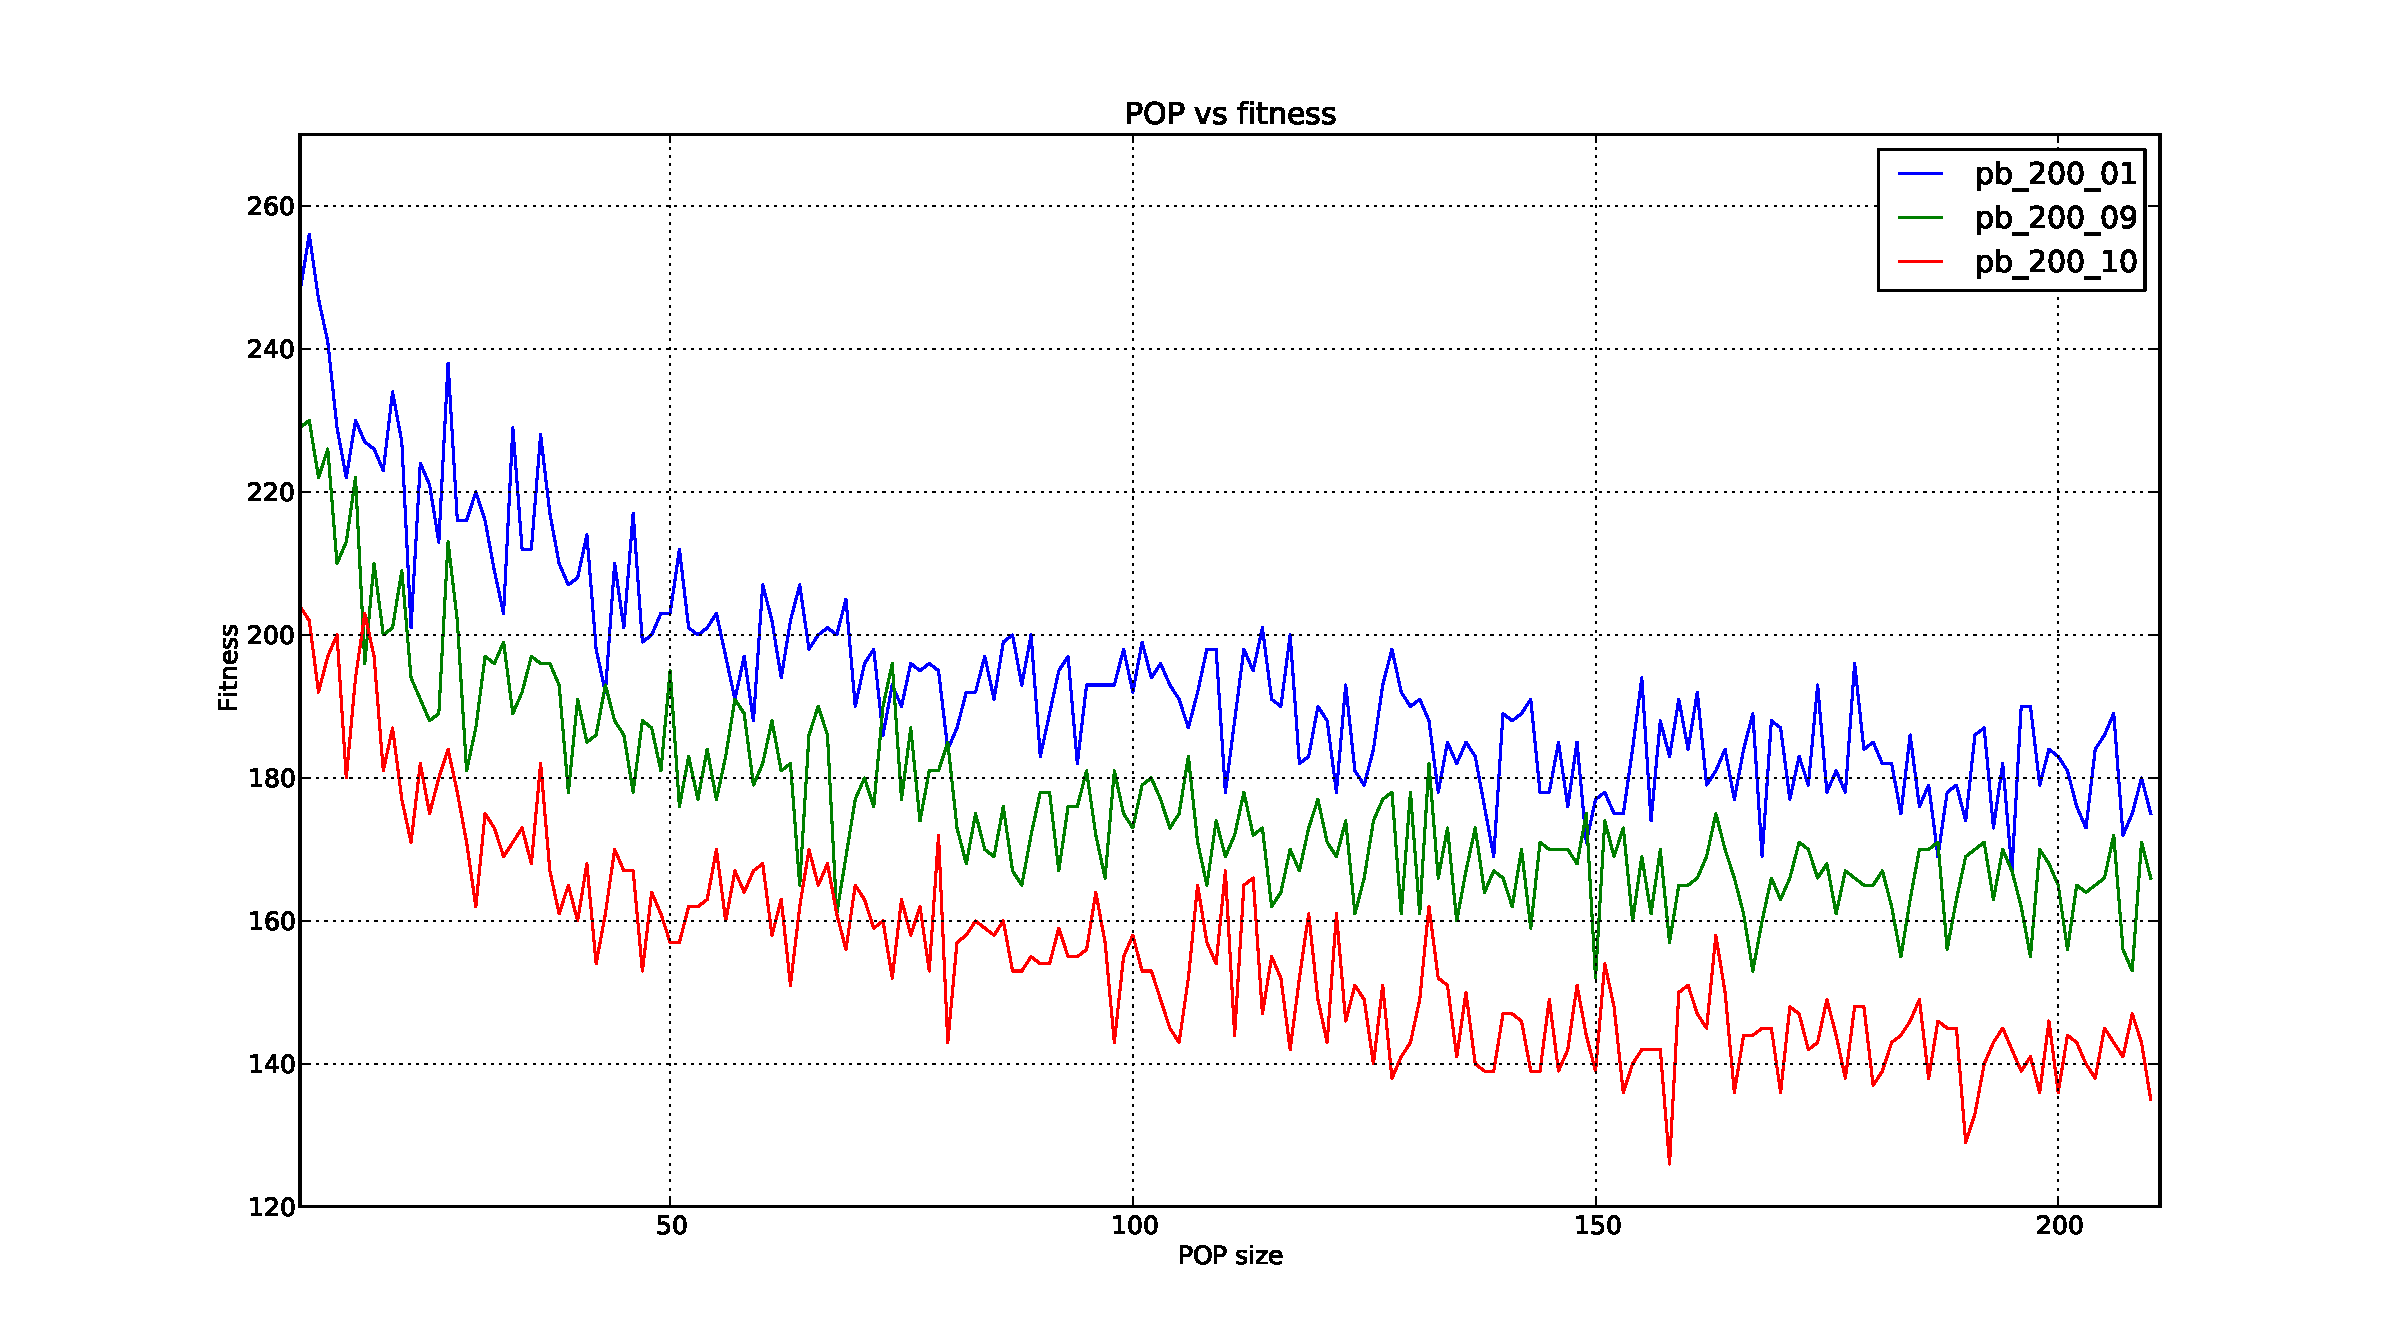
\includegraphics[width=0.95\textwidth]{../doc/img/1.pdf}
\end{center}
}

\frame
{
\frametitle{Sintonización Manual}
\framesubtitle{Prueba 1}
\begin{center}
\begin{tabular}{|l|c|c|c|c|}
    \hline
    \textbf{Instancia} & \textbf{POP} & \textbf{F} & \textbf{T [s] } & \textbf{T tot [s] }\\\hline
    \texttt{pb\_200\_01.txt} & 195 & 167 & 15.110 & 1608.853 \\\hline
    \texttt{pb\_200\_09.txt} & 150 & 152 & 11.243 & 1593.739 \\\hline
    \texttt{pb\_200\_10.txt} & 158 & 126 & 11.210 & 1662.580 \\\hline
\end{tabular}
\end{center}
}


\frame
{
\frametitle{Sintonización Manual}
\framesubtitle{Prueba 2}

\vspace{1cm}
\begin{center}
    Número de generaciones \texttt{(GENS)}
\end{center}
}

\frame
{
\frametitle{Sintonización Manual}
\framesubtitle{Prueba 2}

\begin{center}
    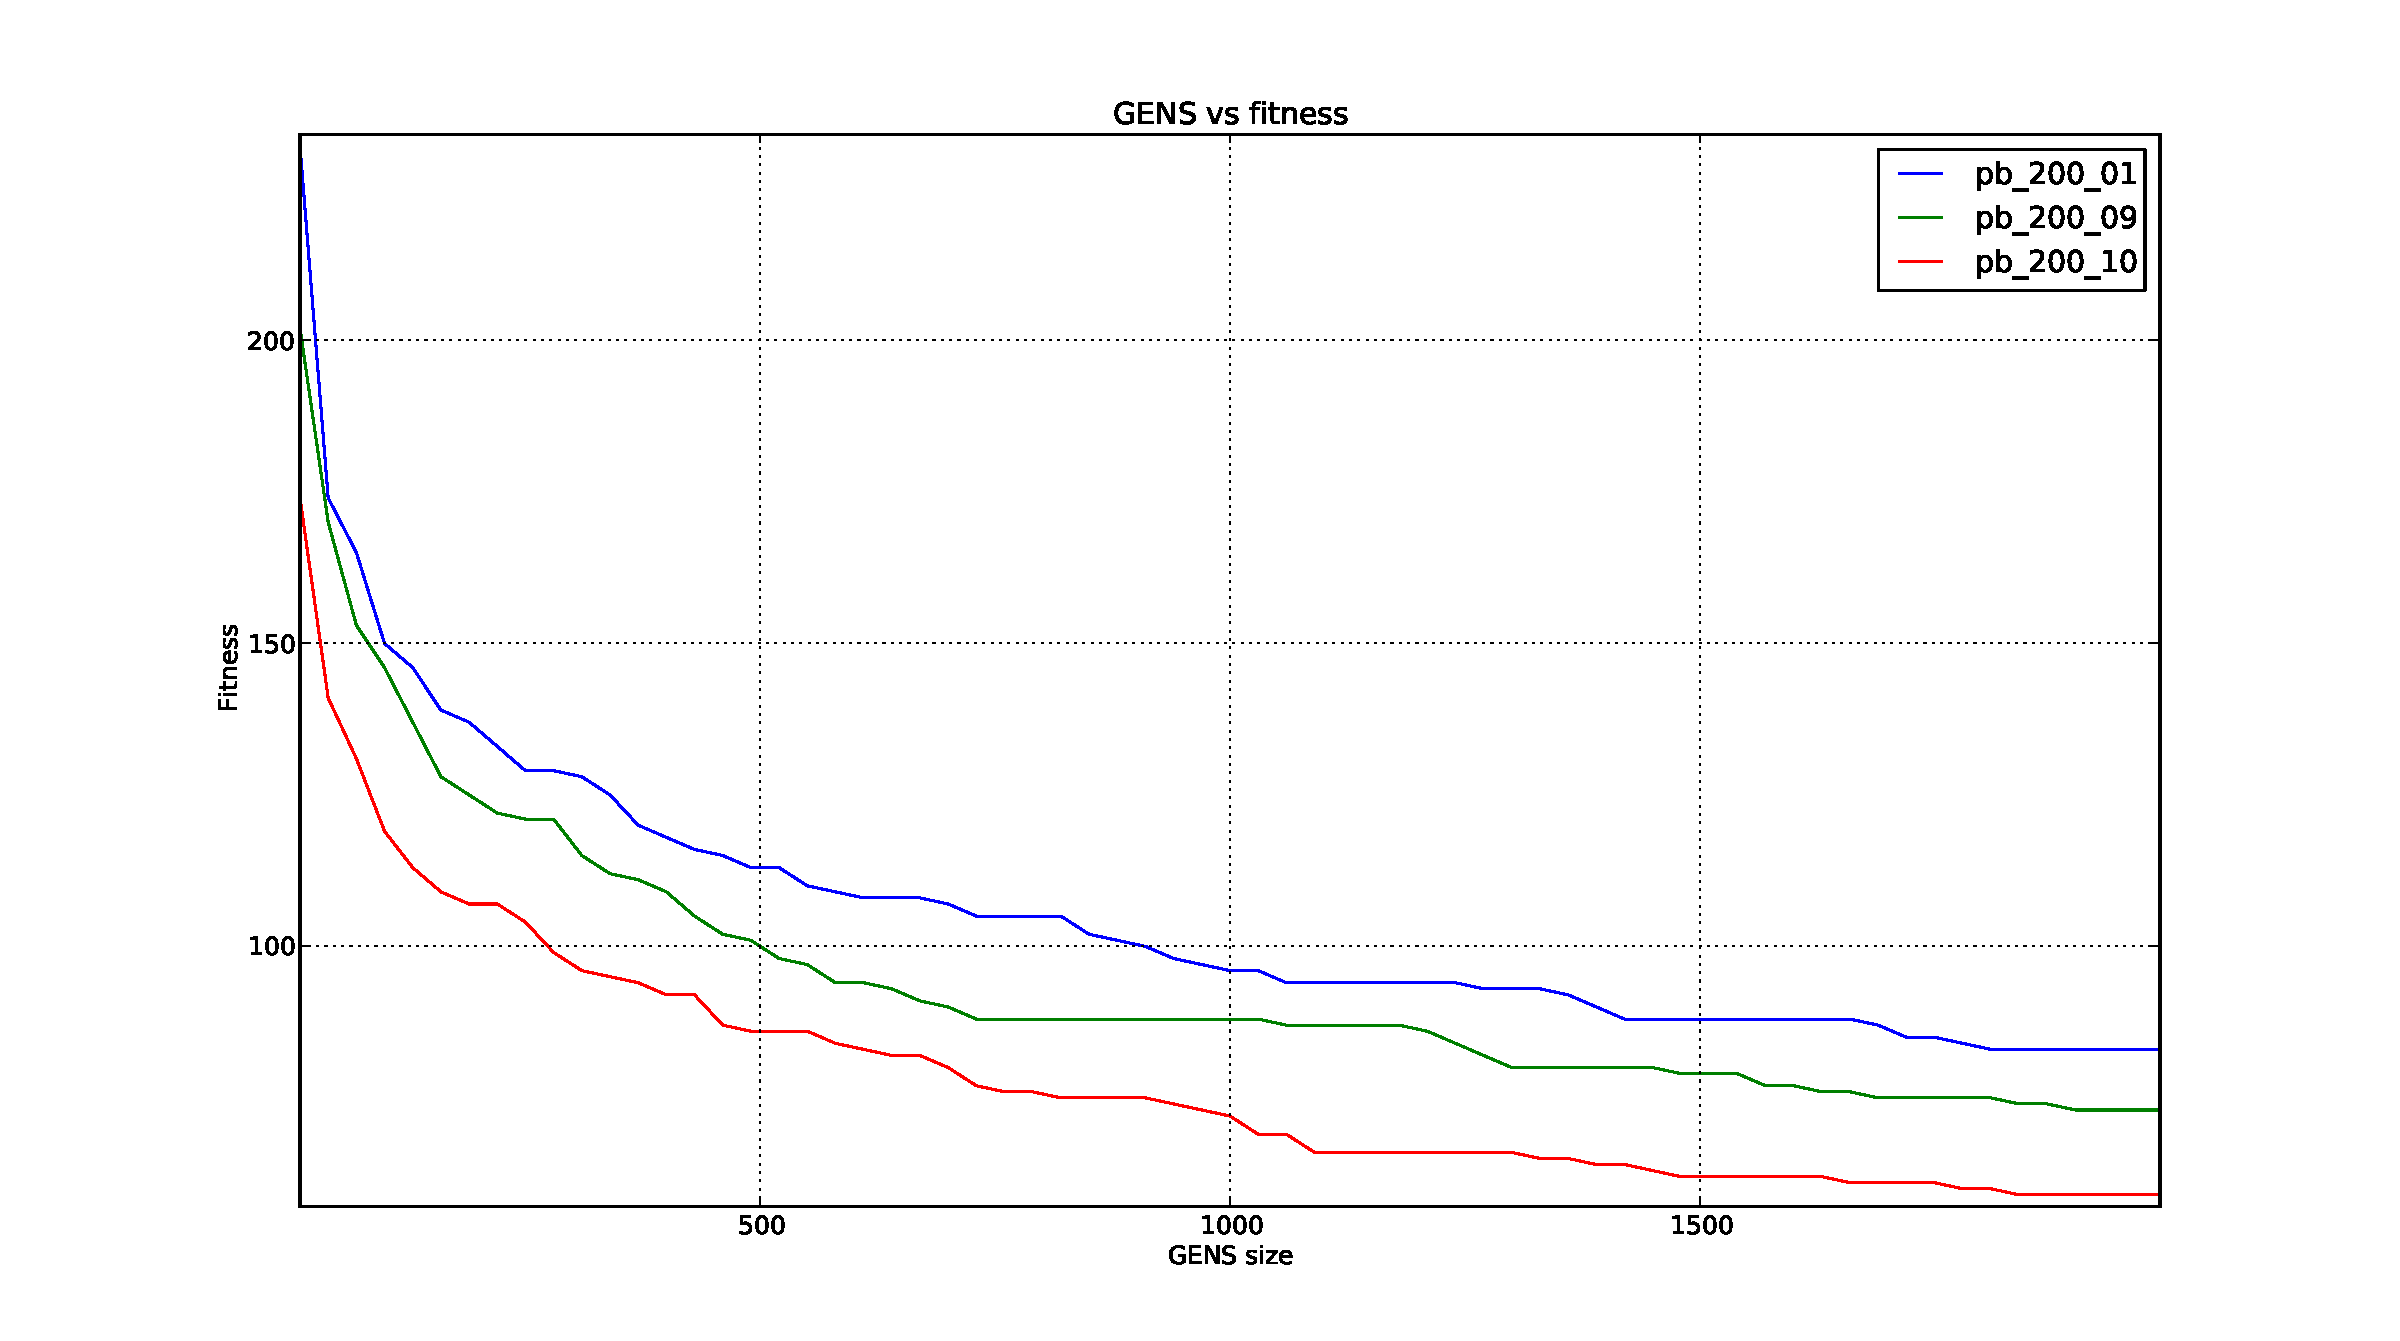
\includegraphics[width=0.95\textwidth]{../doc/img/2.pdf}
\end{center}
}

\frame
{
\frametitle{Sintonización Manual}
\framesubtitle{Prueba 2}
\begin{center}
\begin{tabular}{|l|c|c|c|c|}
    \hline
    \textbf{Instancia} & \textbf{GENS} &\textbf{F} & \textbf{T [s] } & \textbf{T tot [s]}\\\hline
    \texttt{pb\_200\_01.txt} & 1810 & 186 & 7.782 & 256.177 \\\hline
    \texttt{pb\_200\_09.txt} & 1960 & 166 & 8.460 & 262.906 \\\hline
    \texttt{pb\_200\_10.txt} & 1630 & 144 & 7.562 & 256.546 \\\hline
\end{tabular}
\end{center}
}


\frame
{
\frametitle{Sintonización Manual}
\framesubtitle{Prueba 3}

\vspace{1cm}
\begin{center}
    Tasa de reemplazo \texttt{(replaceRate)}
\end{center}
}

\frame
{
\frametitle{Sintonización Manual}
\framesubtitle{Prueba 3}

\begin{center}
    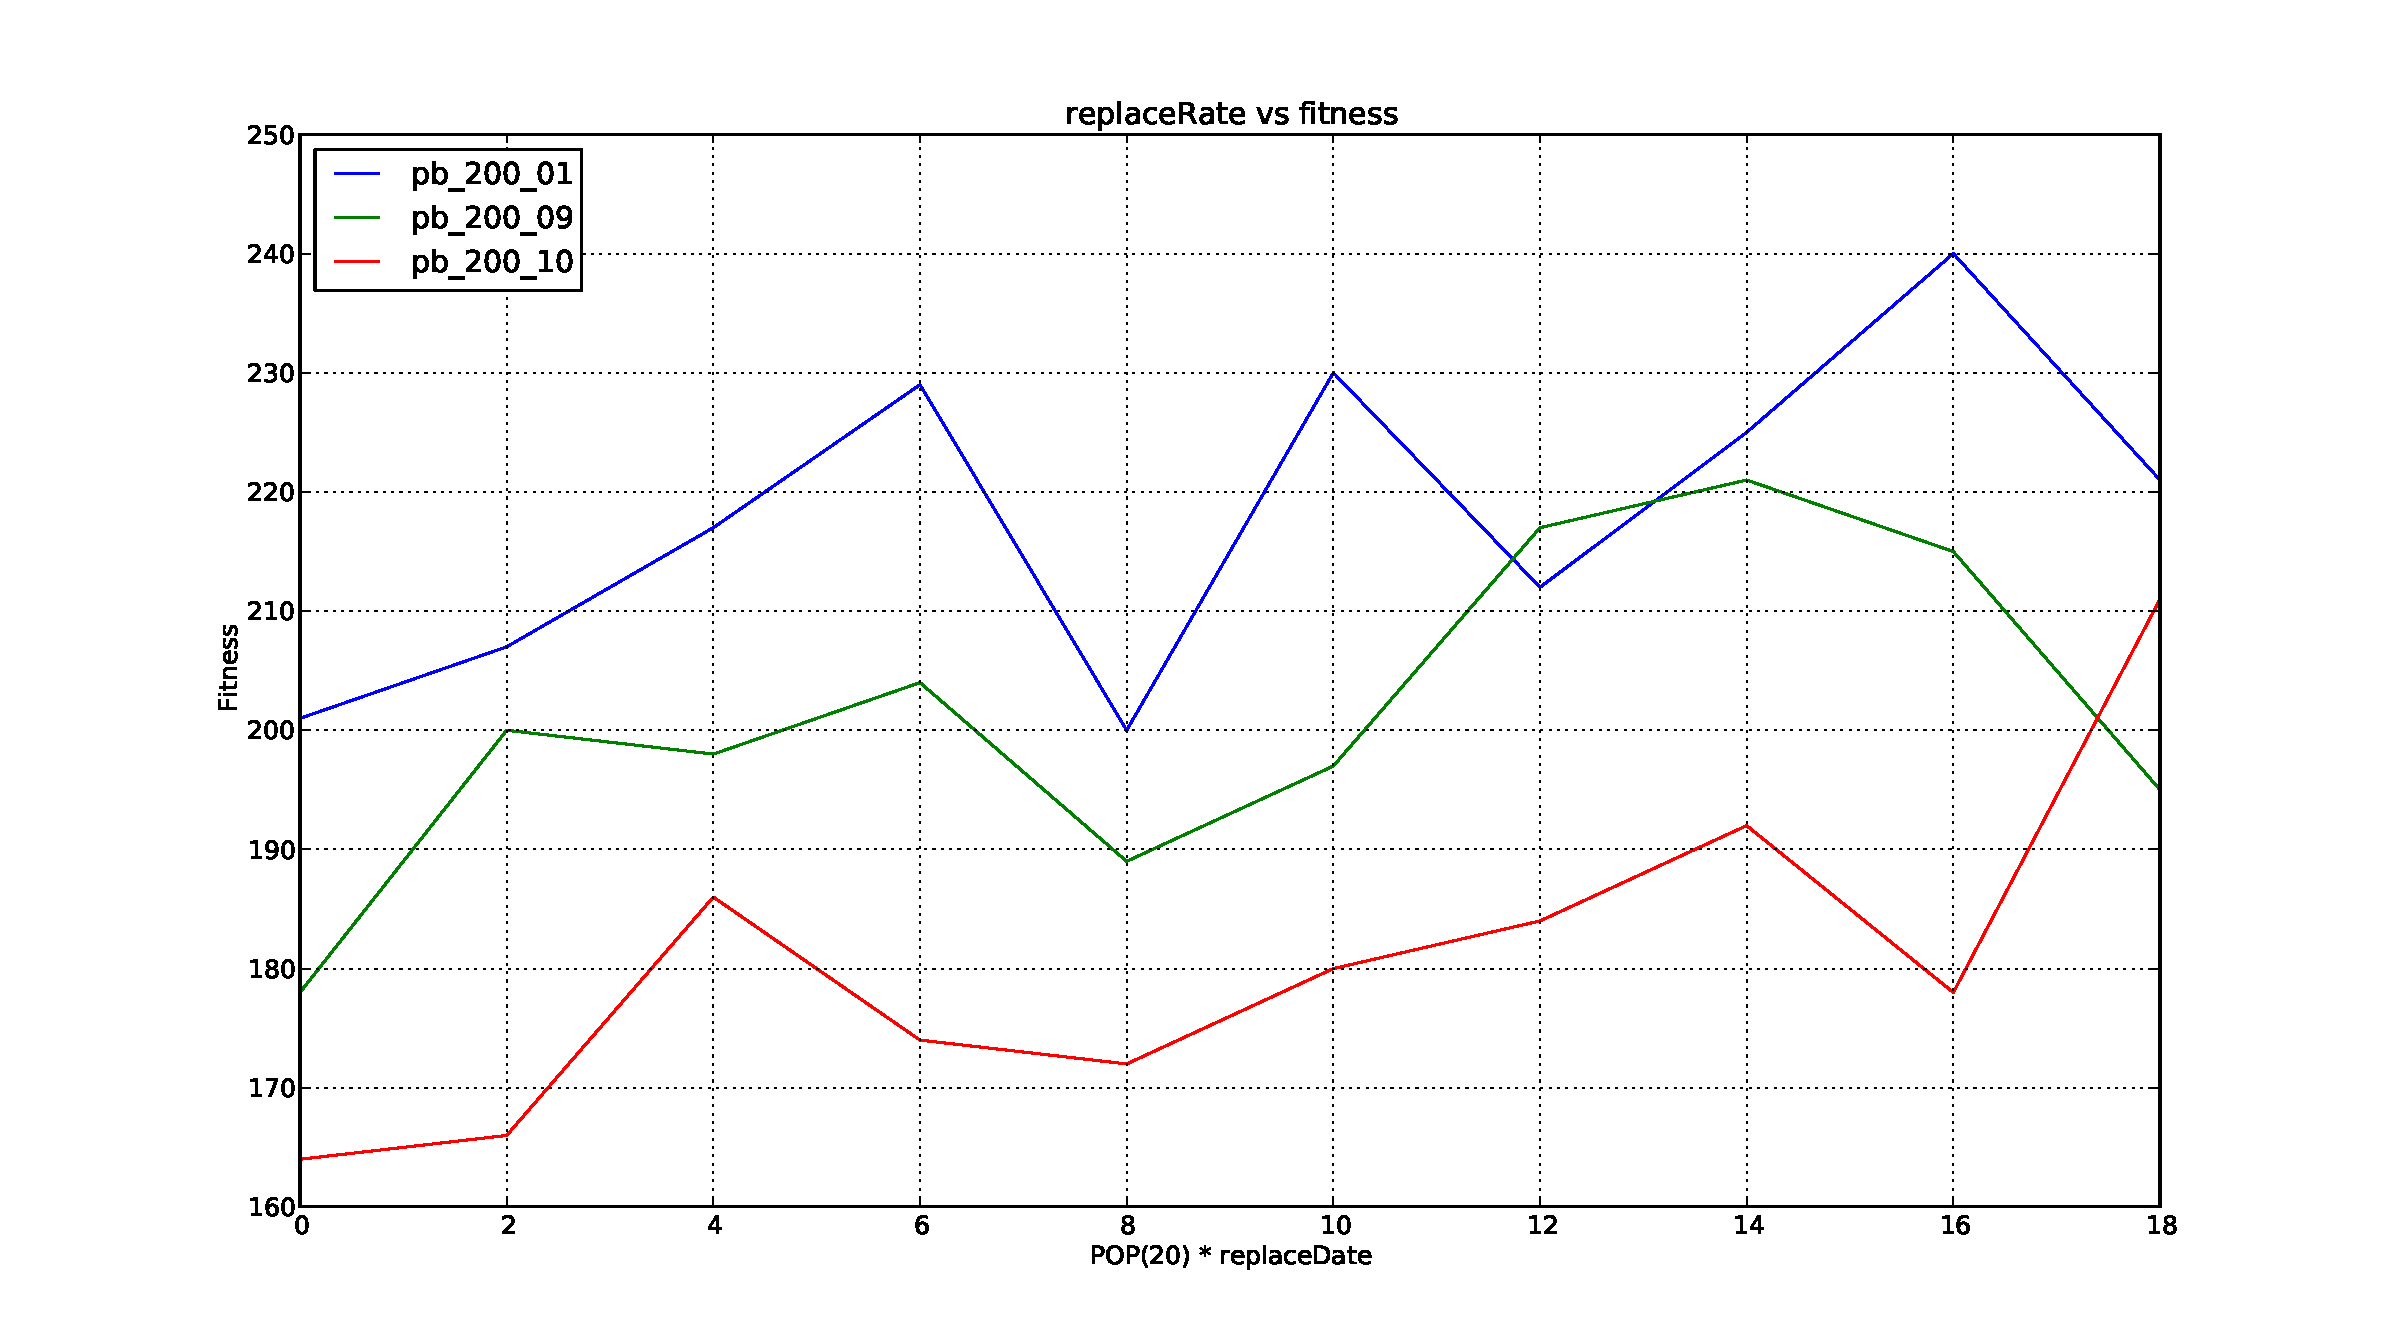
\includegraphics[width=0.95\textwidth]{../doc/img/3.pdf}
\end{center}
}


\frame
{
\frametitle{Sintonización Manual}
\framesubtitle{Prueba 3}
\begin{center}
\begin{tabular}{|l|c|c|c|c|}
    \hline
    \textbf{Instancia} & \textbf{POP*replaceRate} & \textbf{F} & \textbf{T [s]} & \textbf{T tot [s]}\\\hline
    \texttt{pb\_200\_01.txt} & 8 & 200 & 1.374 & 13.246 \\\hline
    \texttt{pb\_200\_09.txt} & 0 & 178 & 1.463 & 12.027 \\\hline
    \texttt{pb\_200\_10.txt} & 0 & 164 & 0.515 & 12.133   \\\hline
\end{tabular}
\end{center}

}

\frame
{
\frametitle{Sintonización Manual}
\framesubtitle{Prueba 4}

\vspace{1cm}
\begin{center}
    Tasa de clonación (\texttt{clonationRate}) y Factor de clonación (\texttt{clonationFactor}).
\end{center}
}
\frame
{
\frametitle{Sintonización Manual}
\framesubtitle{Prueba 4}

\begin{center}
    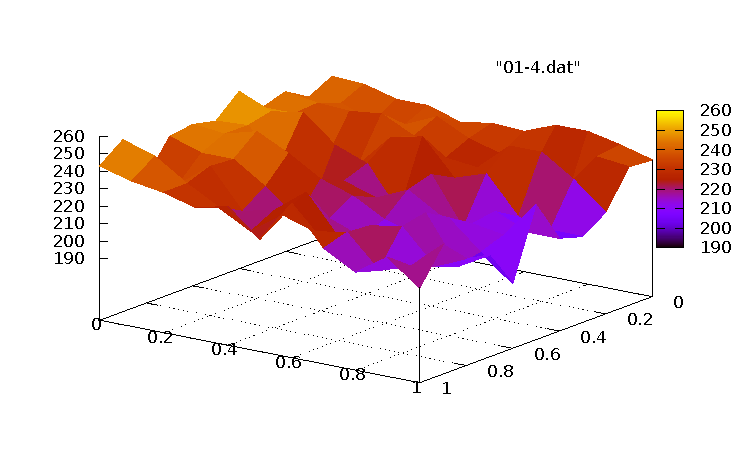
\includegraphics[width=0.95\textwidth]{../doc/img/01-4.pdf}
\end{center}
}

\frame
{
\frametitle{Sintonización Manual}
\framesubtitle{Prueba 4}

\begin{center}
    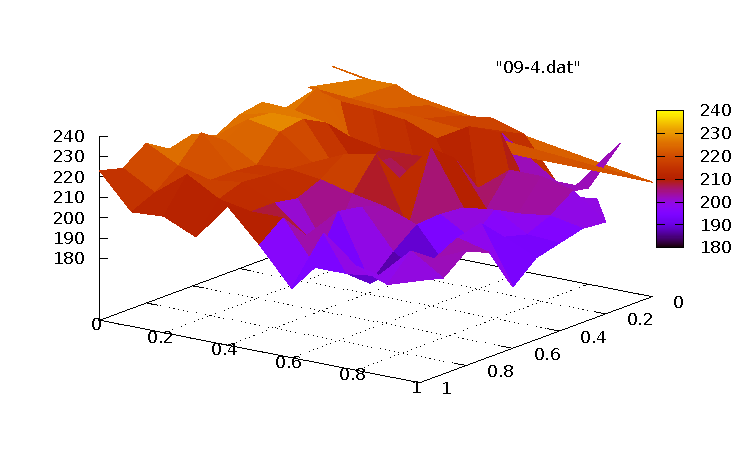
\includegraphics[width=0.95\textwidth]{../doc/img/09-4.pdf}
\end{center}
}

\frame
{
\frametitle{Sintonización Manual}
\framesubtitle{Prueba 4}

\begin{center}
    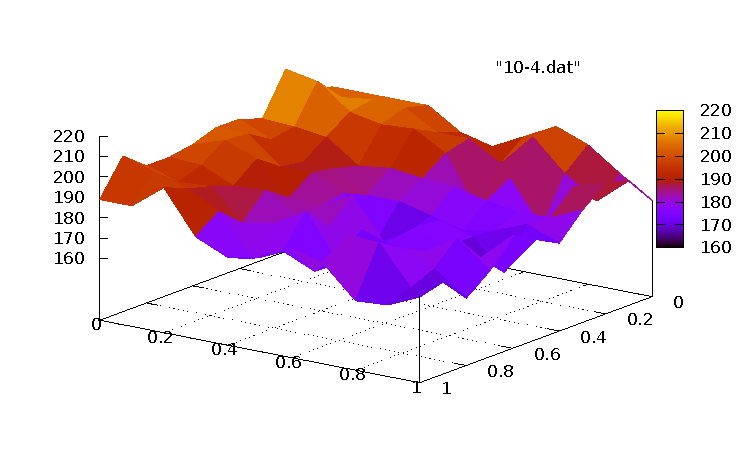
\includegraphics[width=0.95\textwidth]{../doc/img/10-4.pdf}
\end{center}
}
\frame
{
\frametitle{Sintonización Manual}
\framesubtitle{Prueba 4}
\begin{center}
\begin{tabular}{|l|c|c|c|c|c|}
    \hline
    \textbf{Instancia} & \textbf{cRate} & \textbf{cFactor} &\textbf{F} & \textbf{T [s]} & \textbf{T tot [s]}\\\hline
    \texttt{pb\_200\_01.txt} & 0.6 & 1   & 192 & 1.241 & 132.608 \\\hline
    \texttt{pb\_200\_09.txt} & 0.6 & 1   & 180 & 1.378 & 132.068 \\\hline
    \texttt{pb\_200\_10.txt} & 0.5 & 0.9 & 160 & 1.379 & 132.124 \\\hline
\end{tabular}
\end{center}
}

